\documentclass[12pt,journal,a4paper,twocolumn,final,oneside]{IEEEtran}%final,finalsubmission,

\usepackage{multicol}

\usepackage{color}

\usepackage{subfigure}

 \usepackage[plainpages=false,pdfpagelabels,breaklinks=true,pdfborder=0 0 0]{hyperref} % pagebackref

% \def\pagedeclaration#1{\dotfill\nobreakspace\hyperpage{#1}}
% \def\nomentryend{}
% \def\nomlabel#1{\textbf{#1}\hfil}
% \newcommand*{\eqdeclaration}[1]{%
%   \hyperlink{equation.#1}{(Equation~#1)}%
% }
%
% \renewcommand{\backref}[1]{}
% \renewcommand*{\backrefalt}[4]{%
%   \ifcase #1 %
%     %
%   \or
%     \ \emph{(cited on page #2)}.%
%   \else
%     \ \emph{(cited on pages #2)}.%
%   \fi
% }

\usepackage{rotating}
\usepackage[sort,compress,numbers]{natbib} %round,authoryear


% %% BEGIN: Include label in list of references
% \makeatletter
% \def\mysplit#1)#2\@nil{%
% \def\@mysecondoftwo{#2}%
% \ifthenelse{\equal{@@arg}{#1}}
% {% no year, take everything
% \def\@mycitep{#1}}
% {% take the part until and including year
% \def\mycitep{#1)}}}
%
% \def\@lbibitem[#1]#2{%
% \mysplit#1)@@arg\@nil
% \if\relax\@extra@b@citeb\relax\else
% \@ifundefined{br@#2\@extra@b@citeb}{}{%
% \@namedef{br@#2}{\@nameuse{br@#2\@extra@b@citeb}}}\fi
% \@ifundefined{b@#2\@extra@b@citeb}{\def\NAT@num{}}{\NAT@parse{#2}}%
% \item[\hfil\hyper@natanchorstart{#2\@extra@b@citeb}{[{\mycitep}]}%
% \hyper@natanchorend]%
% \NAT@ifcmd#1(@)(@)\@nil{#2}}
% \makeatother
% % %% END: Include label in list of references

\usepackage{nomencl}
\def\nomname{Glossary}
\makenomenclature

\usepackage{graphicx}

% correct bad hyphenation here
\hyphenation{op-tical net-works semi-conduc-tor SPECjAppServer experi-ments}

% \newcommand{\TODO}[1]{\textcolor{red}{\footnote{\textcolor{red}{#1}}}\marginpar{\textcolor{red}{\scriptsize{TODO}}}}
% \newcommand{\MR}[1]{\textcolor{red}{\footnote{\textcolor{red}{#1}}}\marginpar{\textcolor{red}{\scriptsize{Matthias}}}}
% \newcommand{\WH}[1]{\textcolor{red}{\footnote{\textcolor{red}{#1}}}\marginpar{\textcolor{red}{\scriptsize{Willi}}}}
% \newcommand{\JW}[1]{\textcolor{red}{\footnote{\textcolor{red}{#1}}}\marginpar{\textcolor{red}{\scriptsize{Jan}}}}
% \newcommand{\SF}[1]{\textcolor{red}{\footnote{\textcolor{red}{#1}}}\marginpar{\textcolor{red}{\scriptsize{S\"{o}ren}}}}
% \newcommand{\TODOBOX}[1]{\qquad\newline\fbox{\fbox{\parbox{0.95\columnwidth}{\textbf{\color{red}{%TODO:
% }}\noindent  #1 }}\\[0.1cm]}\marginpar{\textcolor{red}{\scriptsize{TODO}}}}

\usepackage{tipa}
\newcommand{\SLAstic}{\mbox{SLAstic}}
\newcommand{\SLAsticPhonetic}{{\sffamily\mbox{SLAstic}}}
\newcommand{\SLAsticComponent}[1]{\mbox{SLAstic.#1}}
\newcommand{\SLAsticSIM}{\SLAsticComponent{SIM}}
\newcommand{\SLAsticMON}{\SLAsticComponent{MON}}
\newcommand{\SLAsticREC}{\SLAsticComponent{REC}}
\newcommand{\SLAsticCTRL}{\SLAsticComponent{CONTROL}}

% \newcommand{\filename}[1]{\textit{\texttt{\small #1}}}
\newcommand{\opname}[1]{\textit{#1}}
% \newcommand{\opnamesmaller}[1]{\textit{\texttt{\scriptsize #1}}}

\newcommand{\classname}[1]{\textit{#1}}
% \newcommand{\pkgname}[1]{\textit{\texttt{\small #1}}}
\def\@hyph{\hbox{$\hookleftarrow$}} \def\+{\discretionary{\@hyph}{}{}}

\urlstyle{same}
% \usepackage{color}
% \definecolor{mygray}{gray}{.75}
\usepackage{listings}
\lstset{%
        language=JAVA,
        basicstyle=\scriptsize, %\footnotesize,
        identifierstyle={},
        commentstyle=\itshape,
        stringstyle=\emph,
        keywordstyle=\ttfamily,
        numbers=left,
        stepnumber=1,
        tabsize=2,
        numbersep=6.5pt,
        xleftmargin=13pt,
        xrightmargin=10pt,
%        numberstyle=\tiny,
%%        numberblanklines=false,
         frame=single,
%         backgroundcolor=\color{mygray},
        breaklines=true,
%        captionpos=t,
        mathescape=true,
        showspaces=false,
        showtabs=false,
%        columns=spaceflexible,
}
%% Listings Fix for IEEETran (only caption, title still doesn't work!)
\makeatletter
\def\lst@makecaption#1#2{\@makecaption{#1}{#2}{}}
\makeatother

\usepackage{pdfpages}

\begin{document}

%\includepdf[nup=1x1,pages=-]{TRTitelA4-p1}

\setcounter{page}{1}

\title{%
Kieker Architecture%
}

\author{%
Kieker team
}

\maketitle

\begin{abstract}\small
\ldots
\end{abstract}

\section{Tpmon}

\subsection{TpmonController}

\begin{figure}[h]\centering
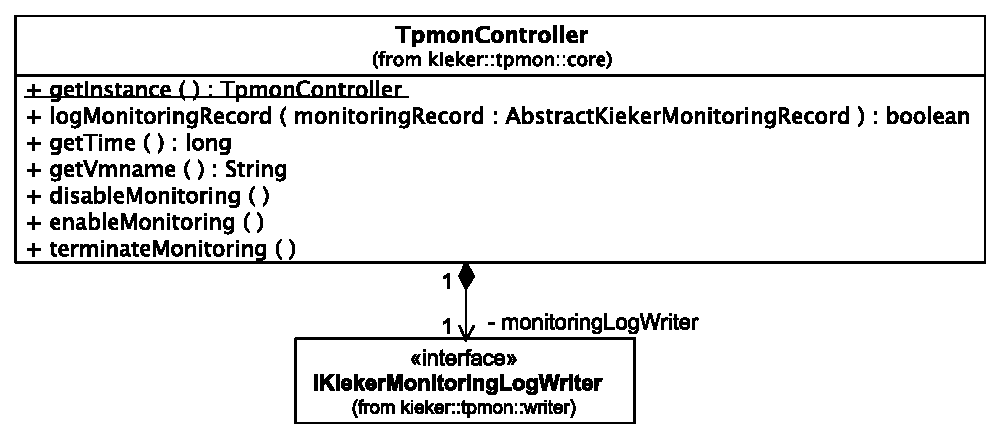
\includegraphics[scale=0.55]{figures/model/kieker_TpmonController}%
\caption{TpmonController}
\end{figure}
 
\subsection{AbstractKiekerMonitoringRecord}

\begin{figure}[h]\centering
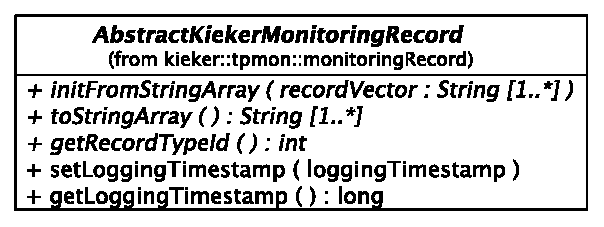
\includegraphics[scale=0.55]{figures/model/kieker_AbstractKiekerMonitoringRecord}%
\caption{AbstractKiekerMonitoringRecord}
\end{figure}

\subsection{KiekerMonitoringLogWriter}

\begin{figure}[h]\centering
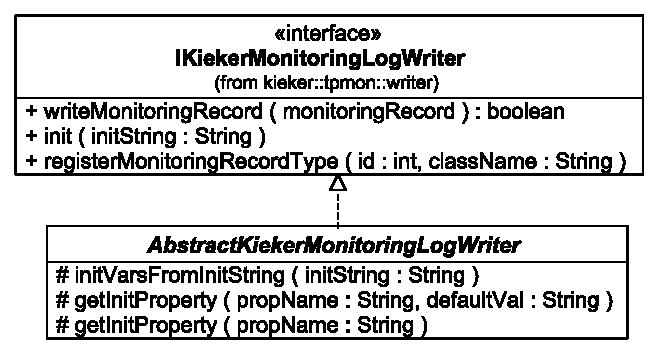
\includegraphics[scale=0.55]{figures/model/kieker_KiekerMonitoringLogWriter}%
\caption{KiekerMonitoringLogWriter}
\end{figure}

\section{Tpan}

\subsection{TpanInstance}



\nocite{vanHoornRohrHasselbringWallerEhlersFreyKieselhorst2009TRContinuousMonitoringOfSoftwareServicesDesignAndApplicationOfTheKiekerFramework,RohrHoornMatevskaStoeverSommerGieseckeHasselbring2008KiekerContinuousMonitoringAndOnDemandVisualizationOfJavaSoftwareBehavior}
\bibliographystyle{unsrtnat-abbrv} %abbrvnat, abbrvnatAvanhoorn % alpha
\bibliography{bibliography}

\end{document}
